\setlist[itemize]{label=\textbullet}
\chapter{Extraction de motifs fréquents à l'aide de l'algorithme Apriori}\label{apriori}
	\section{Introduction}
		\paragraph{}
		Souvent confronté à un ensemble de données qui n'ont vraisemblablement pas une régularité ou des sous structures qui se répètent suivant un certain motif, Une des tâches la plus répandue dans le domaine du Data-Mining est l'extraction de ces dits \textbf{Motifs fréquents}.
		\par 
		De façon informelle, un motifs fréquent peut être un item(objet, article ...) une sous-séquences d'items, une sous-structure(sous-graphe, sous-ensemble ...) qui se répète un certain nombre minimum de fois dans la base de données, ce qui lui vaut le nom de motifs \textbf{fréquent}\cite{Han}.
		\par 
		Dans ce qui suit nous allons voir deux algorithmes capables tout deux d'extraire de tels motifs, l'algorithme \textbf{Apriori} \cite{Agrawal:1994:FAM:645920.672836} et l'algorithme FP-Growth \cite{Hanfp}
		
	\section{Définitions}
		\paragraph{}
		Avant d'introduire les deux algorithmes, il faut d'abord définir quelques concepts qui sont intrinsèquement reliés au déroulement de ces deux derniers:
		\subsection*{Items}
			\paragraph{}
			Un item $I_i$ est généralement un attribut associé à un dataset(Taille,Poids,Catégorie...), cet item a un domaine de définition $D_{I_i}$.
		
		\subsection*{Transaction}\label{transaction}
			\paragraph{}
			Une transaction $T_i$ est généralement une instance du dataset, elle se présente comme un ensemble d'items aux quels une valeur à été attribué : 
			$T_i = \lbrace t_1,t_2,...,t_n\rbrace$, on lui associe un identifiant unique $id_{D_i}$.
		
		\subsection*{Support}
			\paragraph{}
			Un support $S$ est un indicateur(une mesure) de combien de fois un ensemble d'item $X$ apparaît dans un dataset $T$, il est définie comme le nombre de transactions $t$ qui contiennent l'itemset $X$ : 
		
			\begin{equation*}
				Support(X) = \frac{|t \in T ; X \subseteq t|}{|T|}
			\end{equation*}
		
	\section{Algorithme}
		\paragraph{}
		Apriori est un algorithme proposé par Agrawal et Srikant en 1994 dans \cite{Agrawal:1994:FAM:645920.672836}, son but est l'extraction de motifs fréquents dans une base de données de transactions \ref{transaction}.
		\par Apriori construit les ensembles d'items candidats à partir d'un ensemble d'items singletons en générant à chaque itérations une extension de ces derniers en ajoutant un item à la fois tout en testant la condition de support minimum ainsi que la condition de sous-motifs fréquent \footnote{Si $M$ est un motif fréquent alors $\forall m_i \in M $ $m_i$ est aussi un item fréquent} pour permettre l'élimination plus rapide des itemsets candidats, l'algorithme s'arrête quand aucune extension ne peut être générée, le pseudo code est le suivant :
		
	
		\begin{algorithm}[H]
			\caption{Apriori}
			\SetKwInOut{Input}{Entrée}\SetKwInOut{Output}{Sortie}
			\SetKwFunction{gen}{GenererCandidats}
			\SetKwFunction{contains}{Contient}
			
			\Input{(T : Ensemble des transactions , $Sup_{min}$ : entier )}
			\Output{(L : Ensemble des items fréquents)}
			\textbf{Var :} \\
			$C_k : $ Itemset des candidats de taille $K$
			$L_k : $ Itemset des items les plus fréquents de taille $K$
			
			
			\Begin
			{
				$L_1$ \gets $\lbrace items les plus fréquent \rbrace$ ;\\
				\For{($k \gets $ ; $L_k \neq \emptyset $ ; $k \gets k+1$)}
				{
					$L_{k+1} \gets $ \gen{$L_k$};\\
					\ForEach{transaction $t \in T$ }
					{
						\For{candidat $c \in C_{k+1}$}
						{
							\If{\contains{$t$,$c$}}
							{
								$compteur[c] \gets compteur[c]+1$
							}
						}
						
					}
					$L_{k+1} \gets \lbrace 	c | c \in C_{k+1} \land compteur[c] \geq Sup_{min}\rbrace$ 	
				}
				
			}
			\KwRet{$\bigcup\limits_{m} L_m ; m = 0,k $}
		\end{algorithm}
	\section{Implémentation}
		
			\paragraph{}
			Le module \textbf{Apriori} se décompose principalement de trois parties : 
			\begin{itemize}
				\item \textbf{Chargement des données} : la phase où l'on récupère une instance d'un jeu de donnée à travers un fichier d'extension \textbf{.arff} qui contiendra les données et les méta-donnés associée (Nombre d'attributs, leurs types, valeurs manquantes ...), les chargeant en mémoire pour le traitement suivant.
				\item  \textbf{Traitement sur les données} : c'est le coeur du système, c'est ici que l'algorithme va extraire les connaissances souhaitées en appliquant l'algorithme mentionné dans (REFEREEEEEEEEEENCE TO APRIORI), les détails de l'implémentation seons mentionner 
			\end{itemize}
			\par 
			Pour se faire nous avons implémenté 3 classes \textbf{Java} qui effectuent chacune un travail bien précis, communiquant son résultat à une classe. Un diagramme récapitulatif est présenté ici suivi d'une explication sur le fonctionnement de chacune des classes(avec les structures de données qu'elles manipulent)
				
			
			\begin{figure}[H]
				\centering
				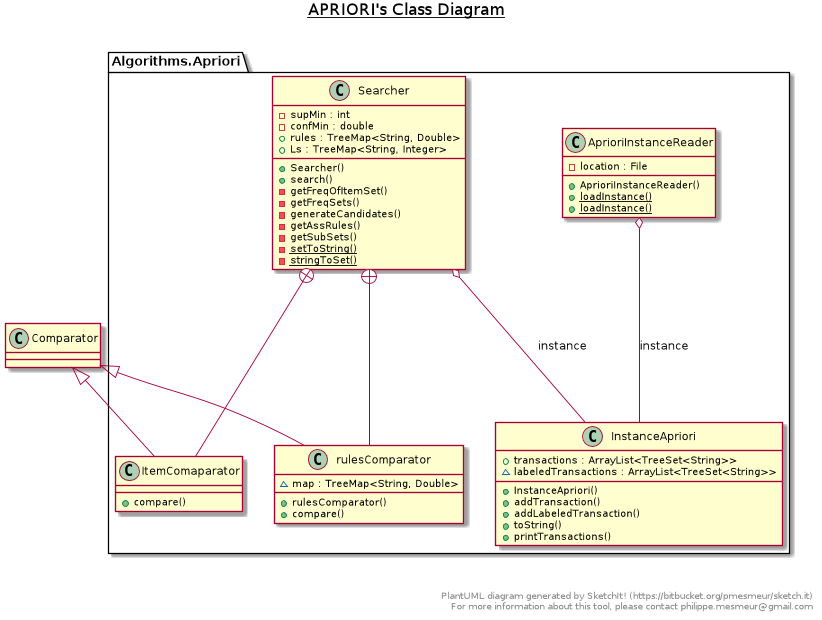
\includegraphics[width=0.75\linewidth]{apriori/images/uml.png}
			\end{figure}
			\paragraph{}
			Pour une vision plus abstraite de ce diagramme , le schéma suivant est proposé : 
			\begin{figure}[H]
				\centering
				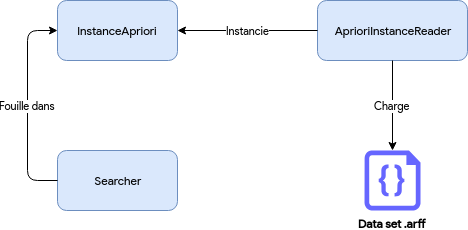
\includegraphics[width=0.75\linewidth]{apriori/images/apriori_schema.png}
			\end{figure}
		
			\subsection*{InstanceApriori : } c'est la classe qui va contenir l'ensemble des transactions ainsi que les méthodes manipulant, les attributs sont les suivants : \\
			\begin{figure}[H]
				\centering
				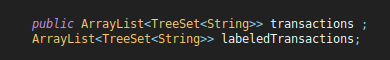
\includegraphics[width=0.75\linewidth]{apriori/images/data_structs/instance/properties.png}
			\end{figure}
			\par 
			Le choix de la structure \textbf{TreeSet} garantie un accès, ajout et suppression d'une entrée en $O(log(n))$, les transactions seront donc représenté comme un vecteur d'ensemble de chaînes de caractères. la différence entre les deux attributs(attribut au sens Orienté-Objet) est que le 2e contient des ensemble de transactions de la forme \textbf{<attribut:valeur\_attribut>}, c'est cette représentation qui sera choisie pour le traitement, l'autre sera utilisé pour l'affichage car il ne dispose pas de l'information sur l'attribut
			\par Pour ce qui en est des méthodes utilisées : 
			\begin{figure}[H]
				\centering
				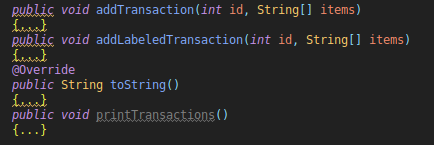
\includegraphics[width=0.75\linewidth]{apriori/images/data_structs/instance/methods.png}
			\end{figure}
			\par, les deux premières méthodes \textbf{addTransaction} et \textbf{addLabeledTransaction} font respectivement office d'interface pour ajouter une transaction à l'un des deux attributs (pour assurer une transparence d'utilisation de la classe). Les deux autres méthodes sont des méthodes d'affichage pour un éventuel débogage de l'application.
			
			\subsection*{AprioriInstanceReader :} \label{loader} c'est la classe qui va construire une objet de la classe \textbf{InstanceApriori} à partir d'un fichier d'extension \textbf{.arff}, ou bien à partir d'un objet de la classe \textbf{weka.Instances} classe déjà existant.
			\par Les attributs sont les suivants : 
			\begin{figure}[H]
				\centering
				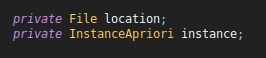
\includegraphics[width=0.75\linewidth]{apriori/images/data_structs/laoder/properties.png}
			\end{figure}
			\par l'attribut \textbf{instances} est donc un objet de la classe \textbf{InstanceApriori} vu précédemment, l'autre est un objet qui stock le descripteur du fichier \textbf{.arff}.
			
			\par 
			Les méthodes sont celles mentionnées dans \ref{loader}, voici leurs prototypes :
			\begin{figure}[H]
				\centering
				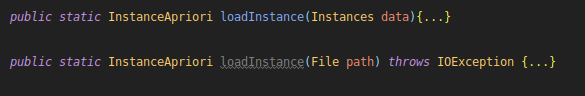
\includegraphics[width=0.75\linewidth]{apriori/images/data_structs/laoder/methods.png}
			\end{figure}
			
			\subsection*{Searcher :} 
			Cette classe est celle qui va contenir à la fois les données en entré (Instance et ses méta-donnés), les hyper paramètres ainsi que le résultat de l'algorithme (Itemsets fréquents et règles d'association).
			\par
			Les attributs sont les suivants 
			\begin{figure}[H]
				\centering
				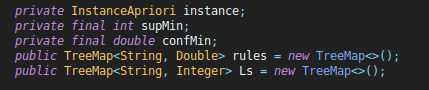
\includegraphics[width=0.75\linewidth]{apriori/images/data_structs/searcher/props.png}
			\end{figure}
			\par Les trois premiers sont triviaux (voir \ref{loader}), les deux derniers sont respectivement : une structure de hachage de la règle d'association à son degré de confiance \textbf{Règle -> Confiance} pour l'attribut \textbf{rules}, et une structure de hachage d'un itemset à sa fréquence d'apparition \textbf{Itemset -> Support}, et cela pour garantir un accès directe l'information désirée.
			
			\par 
			Pour ce qui est des méthodes, il en existe trois catégories :
			\begin{itemize}
				\item \textbf{Méthode principale} : essentiel au fonctionnement de l'algorithme. La seule méthode répondant à cette description est la méthode \textbf{search} : 
				\begin{figure}[H]
					\centering
					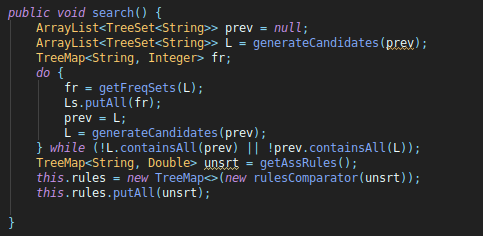
\includegraphics[width=0.6\linewidth]{apriori/images/data_structs/searcher/search.png}
				\end{figure}
				\item \textbf{Méthode d'aide} : pour modulariser le traitement d'une méthode principale, les méthodes suivantes ont font partie : 
				\begin{figure}[H]
					\centering
					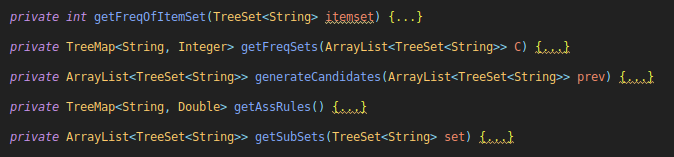
\includegraphics[width=0.75\linewidth]{apriori/images/data_structs/searcher/helpers.png}
				\end{figure}
				\par Dans l'ordre le rôle de chacune est le suivant :
				\begin{itemize}
					\item \textbf{getFreqOfItemSet} Calcule le support d'un itemset
					\item \textbf{getFreqSets} Extrait les itemset fréquents ( dont le support dépasse le support minimum)
					\item \textbf{generateCandidates} Génère un nouveau itemset candidat en combinant les item d'un itemset antérieur.
					\item \textbf{getAssRules} Extrait les règles d'association à partir des itemset fréquents extraits au préalable.
					\item \textbf{getSubSets} Extrait l'ensemble des parties d'ensemble d'un itemset. 
				\end{itemize}
				\item \textbf{Méthode deboggage} : principalement servant à afficher de manière structurée les résultats finaux ou intermédiaire d'un des types de méthodes cités. Nous y trouvons les méthodes : 
				\begin{figure}[H]
					\centering
					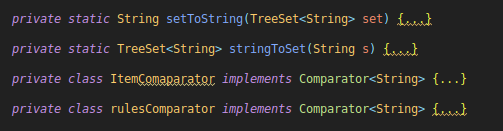
\includegraphics[width=0.75\linewidth]{apriori/images/data_structs/searcher/printers.png}
				\end{figure}
			\end{itemize}
		
	\section{Interface graphique}
		\paragraph{}
		Nous avons intégré l'interface graphique pour l'utilisation d'algorithme \textbf{Apriori} dans l'interface principale, pour que l'utilisateur puisse lancer le traitement sur une datase préalablement traité (nettoyage et remplissage de valeur manquantes), voici l'interface choisie suivit de quelques explications : 
		\begin{figure}[H]
			\centering
			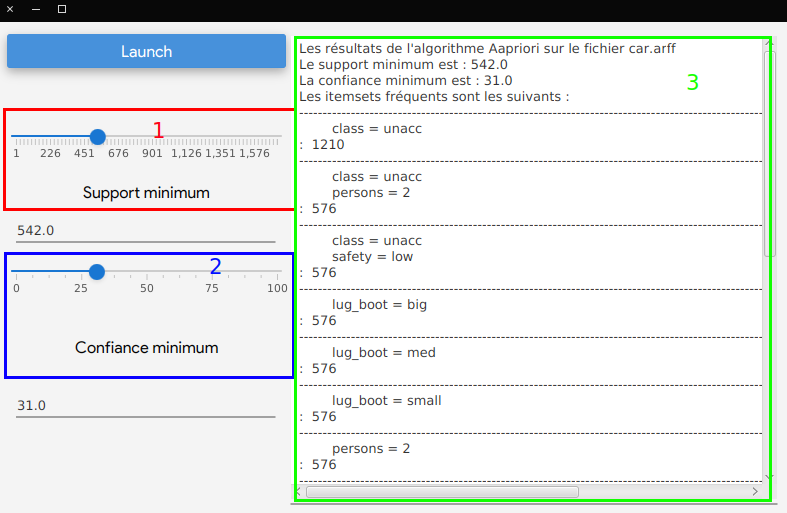
\includegraphics[width=0.75\linewidth]{apriori/images/apriori.png}
		\end{figure}
		\paragraph{}
		L'interface se compose de 3 zones :
		\begin{itemize}
			\item \textbf{Zone 1 et 2:} permettre d'introduire les valeurs des hyper paramètres
			\item \textbf{Zone 3:} affichage du résultat comme une liste d'itemsets fréquents suivie d'une liste de règle d'association. 
		\end{itemize}
		
	\section{Résultats expérimentaux}
		\subsection{Choix du dataset}
			\paragraph{}
			Pour tester le comportement de notre implémentation de l'algorithme apriori, nous avons choisi de le tester sur un dataset purement nominal (\textbf{car.arff}).
		\subsection{Variations des paramètres}
			\paragraph{}
			Nous avons choisi de faire varier les deux paramètres qui sont supMin et confMin de façon automatique, la plage du premier est l'intervalle $\left[ \text{0.1*\textbf{nombreInstance} , \textbf{nombreInstance}} \right]$ avec un pas $step = \frac{ nombreInstance}{10}$.
			\par 
			La plage du 2e est l'intervalle suivant : $\left[ 0.5 , 1\right]$ avec un pas $step = 0.1$
		\subsection{Résultats}
			\paragraph{}
			Les résultats sont récapitulé dans le tableau suivant : 
			% Please add the following required packages to your document preamble:
			% \usepackage[table,xcdraw]{xcolor}
			% If you use beamer only pass "xcolor=table" option, i.e. \documentclass[xcolor=table]{beamer}
			\begin{table}[H]
				\centering
				\begin{tabular}{|c|c|c|c|c|}
					\hline
					\textbf{supMin} & \textbf{confMin} & \textbf{nombre itemset freq} & \textbf{nombre de règle d'ass} & \textbf{temps (ms)} \\ \hline
					172             & 0.5              & 86                           & 22                             & 410            \\ \hline
					172             & 0.6              & 86                           & 14                             & 431            \\ \hline
					172             & 0.7              & 86                           & 6                              & 433            \\ \hline
					172             & 0.8              & 86                           & 2                              & 388            \\ \hline
					172             & 0.9              & 86                           & 1                              & 382            \\ \hline
					344             & 0.5              & 31                           & 6                              & 41             \\ \hline
					344             & 0.6              & 31                           & 6                              & 42             \\ \hline
					344             & 0.7              & 31                           & 3                              & 44             \\ \hline
					344             & 0.8              & 31                           & 2                              & 40             \\ \hline
					344             & 0.9              & 31                           & 1                              & 47             \\ \hline
					516             & 0.5              & 12                           & 1                              & 36             \\ \hline
					516             & 0.6              & 12                           & 1                              & 39             \\ \hline
					516             & 0.7              & 12                           & 1                              & 38             \\ \hline
					516             & 0.8              & 12                           & 1                              & 37             \\ \hline
					516             & 0.9              & 12                           & 1                              & 39             \\ \hline
					688             & 0.5              & 1                            & 0                              & 43             \\ \hline
					\rowcolor[HTML]{9AFF99} 
					...             & ...              & ...                          & ...                            & ....           \\ \hline
					1204            & 0.9              & 1                            & 0                              & 35             \\ \hline
					\rowcolor[HTML]{9AFF99} 
					...             & ...              & ...                          & ...                            & ...            \\ \hline
					1720            & 0.9              & 0                            & 0                              & 33             \\ \hline
				\end{tabular}
				\caption{Tableau récapitulatif des résultats de l'algorithme apriori sur le dataset \textbf{car.arff}}
				\label{my-label}
			\end{table}
			\paragraph{Remarques :} Les valeurs en vert désignent un stagnation des valeurs \textbf{nombre itemset freq} et \textbf{nombre de règle d'ass}
		\paragraph{Commentaires}
			\paragraph{}
			D'après le tableau, il est notable que le paramètre qui influe le plus sur le temps d'exécutions est le \textbf{support minimum}, c'est facilement remarquable si on prend une valeur fixe pour ce dernier en faisant varier l'autre paramètre \textbf{Confiance minimum}, par exemple : \\
			\[
				\text{Si } supMin = 344 \text{ et } \forall confMin \rightarrow temps \in \left[ 40,47\right]
			\]
			Cela montre que la plus part des ressources sont mobilisé pour l'extraction des itemsets fréquents.
			\par Il est aussi a noté que plus le support minimum augmente ( on impose donc un forte condition sur la fréquence d'apparitions des itemsets) le nombre d'itemsets fréquent ainsi que le nombre de règles d'association ainsi que le temps de calcul diminuent en conséquence.

	